\documentclass[12pt]{beamer}
\usepackage{lmodern}
%\usepackage[german]{babel}
\usepackage[utf8]{inputenc}
\usepackage[T1]{fontenc}
\usepackage[orientation=portrait,size=a0,scale=1.33]{beamerposter} % A0 = 84,1 x 118,9 cm (poster hanger 82 x 117, 10 mm margin => 2.5%)
\usepackage[margin=20mm,padding=20mm,blockspace=0.25\baselineskip]{beamerposterHSNR}
\usepackage{csquotes}
\usepackage{subcaption}
\usepackage
[
	backend=bibtex,
	hyperref=false,
	%style=alpha,
	%citestyle=alpha,
	doi=false,
	isbn=false,
	url=false,
	eprint=false,	
	sorting=nyt,
	giveninits=true
]
{biblatex}

\addbibresource{bib/quix}
\addbibresource{bib/dice1945measures}
\addbibresource{bib/frangi1998multiscale}
\addbibresource{bib/Wibowo2017}

\title{Master Project 2021: Data Lake}
\author{\hspace{1em}\underline{\vphantom{Wy}Alexander Martin, Marcel Thiel, Robin Kuller}} % you can underline the primary author
\affiliations{\hspace{1em}Hochschule Niederrhein, Krefeld, Germany}
\posterdate{February 4, 2021}
\posterconference{Presentation of Master Projects}
\posterlocation{Krefeld, Germany}
\posterlogotopright{
\includegraphics[width=\textwidth]{cd/ipattern}}

\newcommand{\percent}{\raisebox{2pt}{\scalebox{0.825}{\%}}} % properly scaled percent-symbol

\begin{document}
%\usebackgroundtemplate{\includegraphics[width=\paperwidth]{hsnr_background}} % optional: background graphic
\begin{textblock}{0.5}(0.0, 0.0)

% Abstract ---------------------------------------------------------------------------------------------------------
\begin{block}{Abstract}
"Brief Abstract"

Lorem ipsum dolor sit amet, consectetur adipiscing elit. Phasellus iaculis purus eget neque semper, quis dictum est volutpat. Phasellus tempus lacinia velit vitae scelerisque. Nulla lacinia enim eu dui ullamcorper, vitae faucibus libero ultricies. Donec tristique nulla quis massa facilisis, ut posuere arcu ullamcorper. Nulla malesuada velit tortor, a aliquet est consectetur eget. Curabitur tincidunt euismod feugiat. Aliquam velit turpis, posuere nec risus non, sollicitudin accumsan velit. Nullam vitae mi nisi. Duis sed cursus magna.
\end{block}

% Introduction ----------------------------------------------------------------------------------------------------
\begin{block}{Introduction}
"This should include a short background of the topic to set the context and state the main aims and objectives of your piece of work. What differentiates your work from your competition? Why is your work novel in the field?"

Copied from Quix: Data lakes have been proposed as a solution to deal with the heterogeneity of big data, as they should provide a storage system for any kind of raw data. Metadata is of particular importance in such a system to have information about the structure and semantics of the data. The group has been working on the enhancement of the data lake system Constance. It is based on a modular architecture with components for schema matching, schema mapping, query rewriting, and wrapping of data sources. This system is applied in other research projects, e.g., mi-Mappa, HUMIT, and charMAnt, as basic platform for data
\par
\bigskip
\bigskip
Own: Developed our own data lake based on the schemata defined in the shown figure; 
\vspace{1.0\baselineskip}
\begin{wfigure}{1.0}{1}
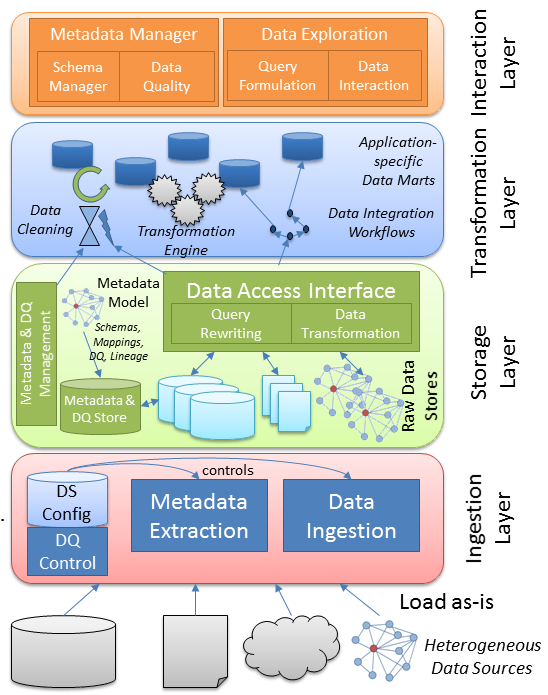
\includegraphics[width=0.75\columnwidth]{graphics/dlarch}
\caption{Data lake architecture[3]}
\end{wfigure}
\hfill
\end{block}

% Methods --------------------------------------------------------------------------------------------------------
\begin{block}{Methods}
"The methods section (poster space permitting) should include basic parameters including target sample, setting, duration of study, inclusion/exclusion criteria, statistical techniques, key interventions assessed and primary outcome measures."

used flask, angular, react, spark and all different kinds of dbs; for easy deployment and scaling we used docker.
\end{block}


\end{textblock}
% Next Column ###########################################################
\begin{textblock}{0.5}(0.5, 0.00)


% Results ----------------------------------------------------------------------------------------------------------
\begin{block}{Results}
"The results section should include data analysis and stratification and should only include the results which answer the stated hypothesis. Moreover, essential to the results section is the inclusion of pertinent and key graphs, graphics, images and tables. These need to be large enough for the audience members to see and be as attractive and clutter-free as possible."
\begin{itemize}
\item Ingestion Layer
\begin{itemize}
\item Own: Ingestion of structured (sql) and semi-structured (json, xml) data is possible; for each ingested dataset a metadata entry is generated (maybe show the schema); 
\end{itemize}
\item Storage Layer
\begin{itemize}
\item Own: The datasets can be stored in their source format and storage-system; For files the default target storage-system is HDFS, for sql it is postgresql and for document-orientated data it is mongodb; However, if the user wants he can select a different target storage-system at his own risk
\end{itemize}
\item Transformation Layer
\begin{itemize}
\item 
\end{itemize}
\item Interaction Layer
\begin{itemize}
\item 
\end{itemize}
\end{itemize} 
\end{block}

% Conclusion -----------------------------------------------------------------------------------------------------
\begin{block}{Conclusion}
"The conclusions must derive directly from the results section and answer solely what has been proposed at the start of the paper. Obvious confounders and limitations should also be acknowledged. Key improvements as well as potential for project expansion should also be considered."
\begin{itemize}
\item Achievements
\begin{itemize}
\item additional components can be included easily
\end{itemize}
\item Confounders / Limitations
\begin{itemize}
\item using Bytestream for uploading files
\end{itemize}
\item Improvements \& Project Expansion
\begin{itemize}
\item Machine-Learning integrated in Apache Spark
\item Data Cleaning
\item Data Quality Check at Ingestion Layer
\item Sharded MongoDB Cluster
\end{itemize}
\end{itemize}
\end{block}

% the bibliography
\vfill\vspace{7.5mm} % at the bottom, but at least some spacing
\begin{block}{References}
"Only cite key references integral to your study, as references are wordy and space consuming. Use a smaller font to the main body text to reduce this."

\nocite{*}
\parbox{\textwidth}{
\AtNextBibliography{\small}
\printbibliography
}
\end{block}

\end{textblock}
\end{document}